\chapter{\textbf{Экспериментальный раздел}}

\hfill

Проводится анализ реализованного приложения, проверяется корректность работы, строятся графики зависимости времени генерации картинки от количества частиц и количества потоков. 

\section{\textbf{Исследование характеристик программы }}

В работе для ускорения вычислений используется параллельной программирование. Необходимо исследовать оптимальное число потоков необходимых для наиболее быстрой генерации изображения. 

Из графика, представленного на рисунке \ref{img:graph} видно, что при генерации частиц, количество которых не превышает 50, использование 4 поток наиболее эффективно, например на 15\% чем 8 потоков и в 4 раза чем при использовании 1 потока. 

Однако при росте числа частиц, ситуация меняется. Использование 8 и 16 потоков становится эффективнее, причем 8 потоков быстрее чем 16 на 3\%. 

\begin{figure}[H]
	\centering
	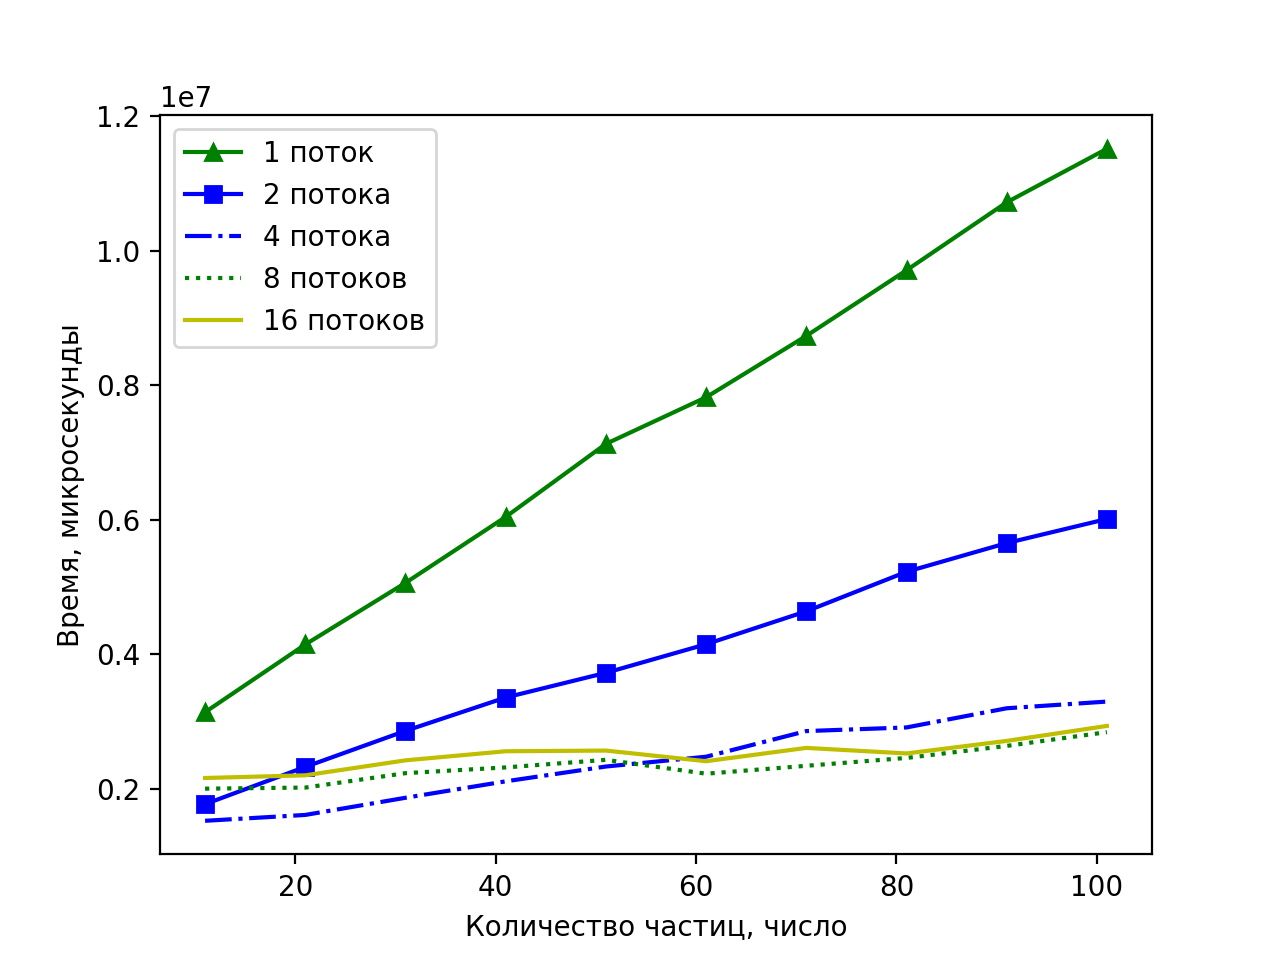
\includegraphics[scale=1]{graph}
	\caption{График зависимости времени генерации изображения от количества частиц для различного числа потоков}
	\label{img:graph}
\end{figure}

Стоит заметить, что 8 потоков соответствует количеству логических ядер процессора. 

Таким образом, получается что количество потоков будет на прямую зависеть от параметров компьютера, на котором запущена визуализация. 

\section{\textbf{Примеры использования программы }}

Примеры работы программы представлены на рисунках \ref{img:ex1}, \ref{img:ex2}. Визуализация одного и того же процесса в разные моменты времени. 

\begin{figure}[H]
	\centering
	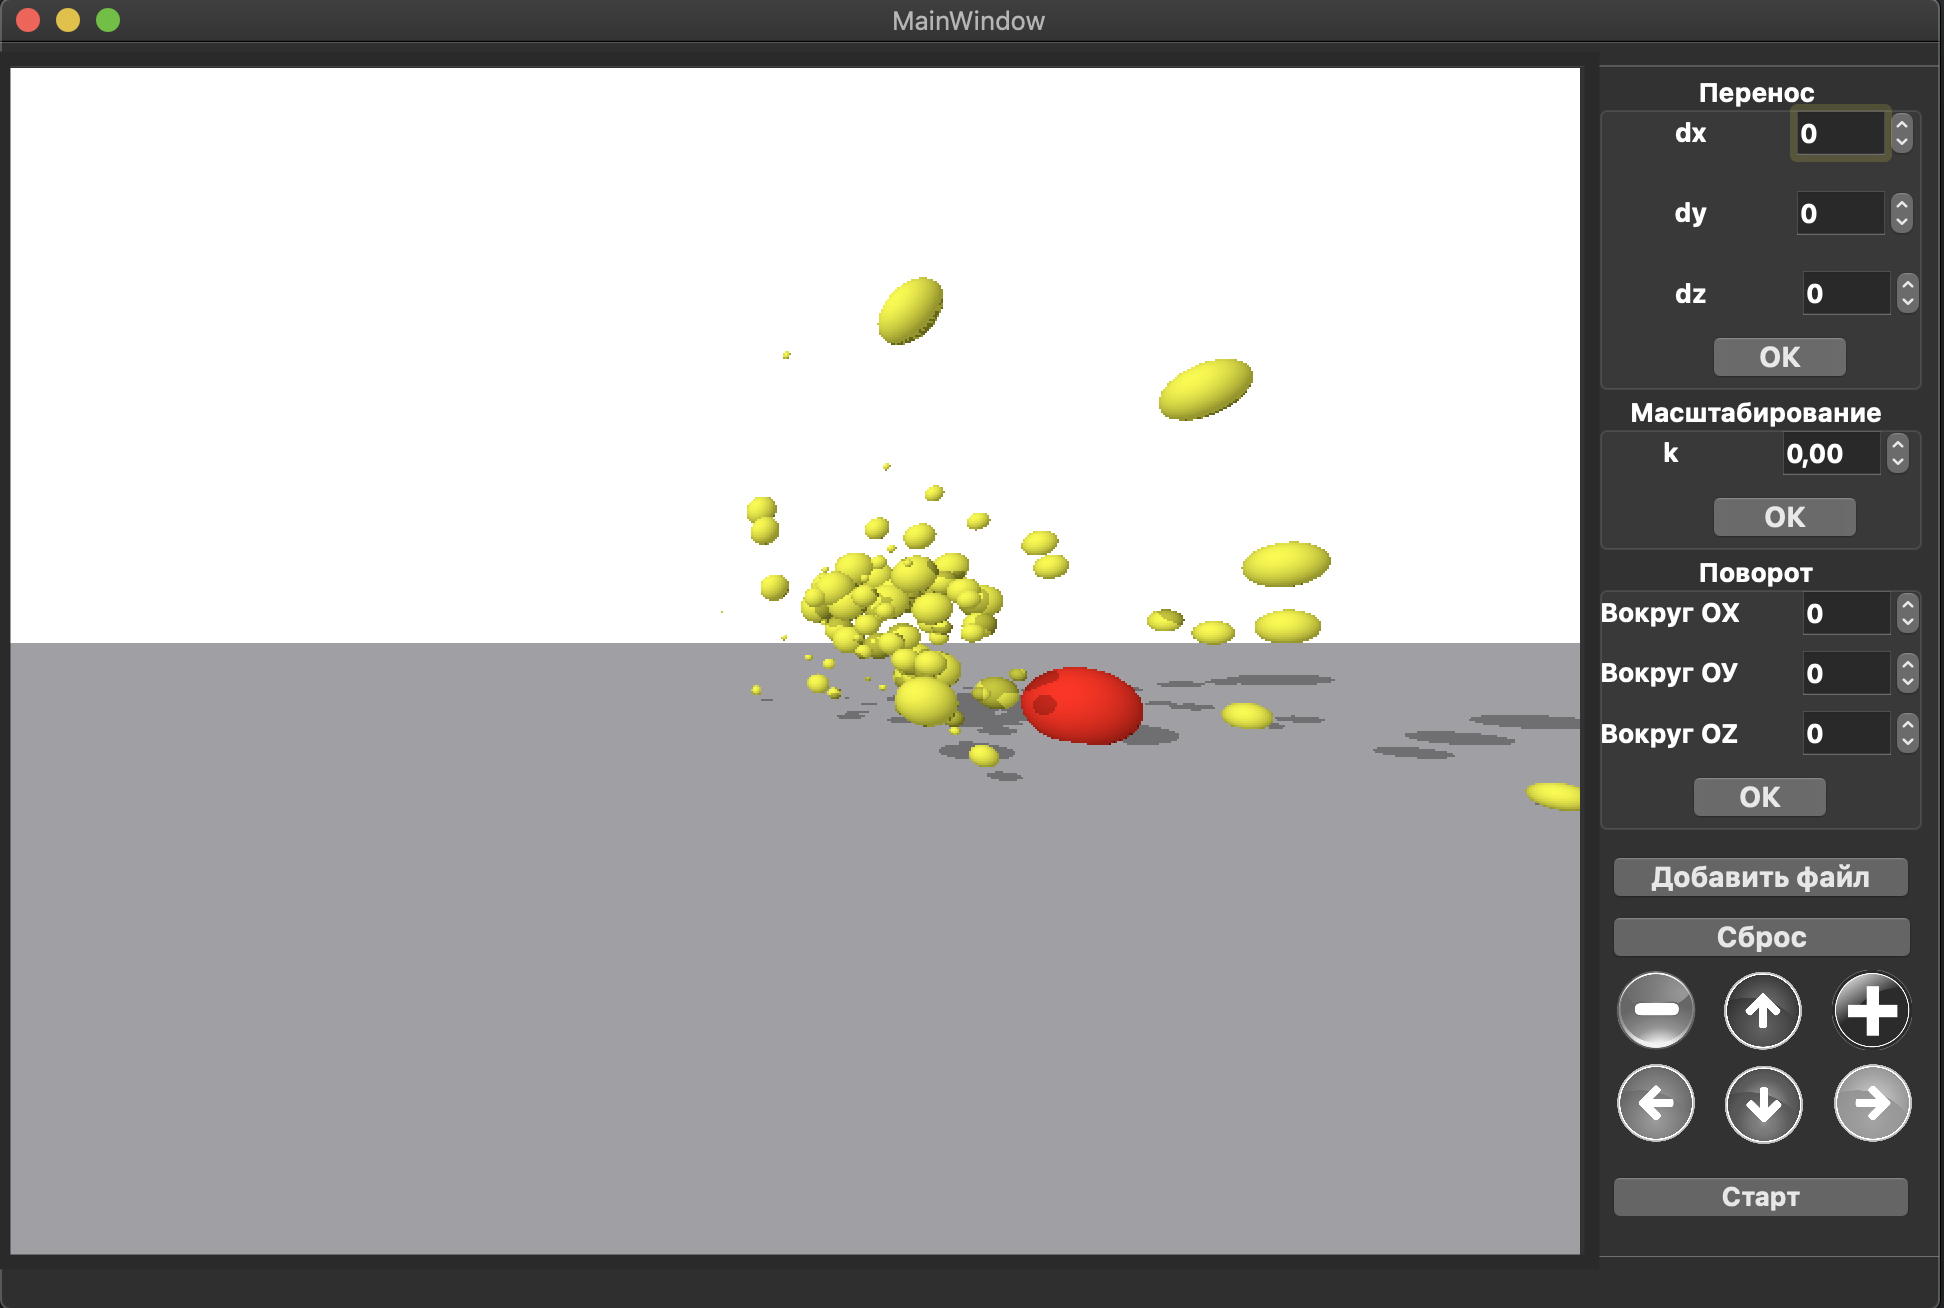
\includegraphics[scale=0.4]{ex1}
	\caption{Пример 1}
	\label{img:ex1}
\end{figure}

\begin{figure}[H]
	\centering
	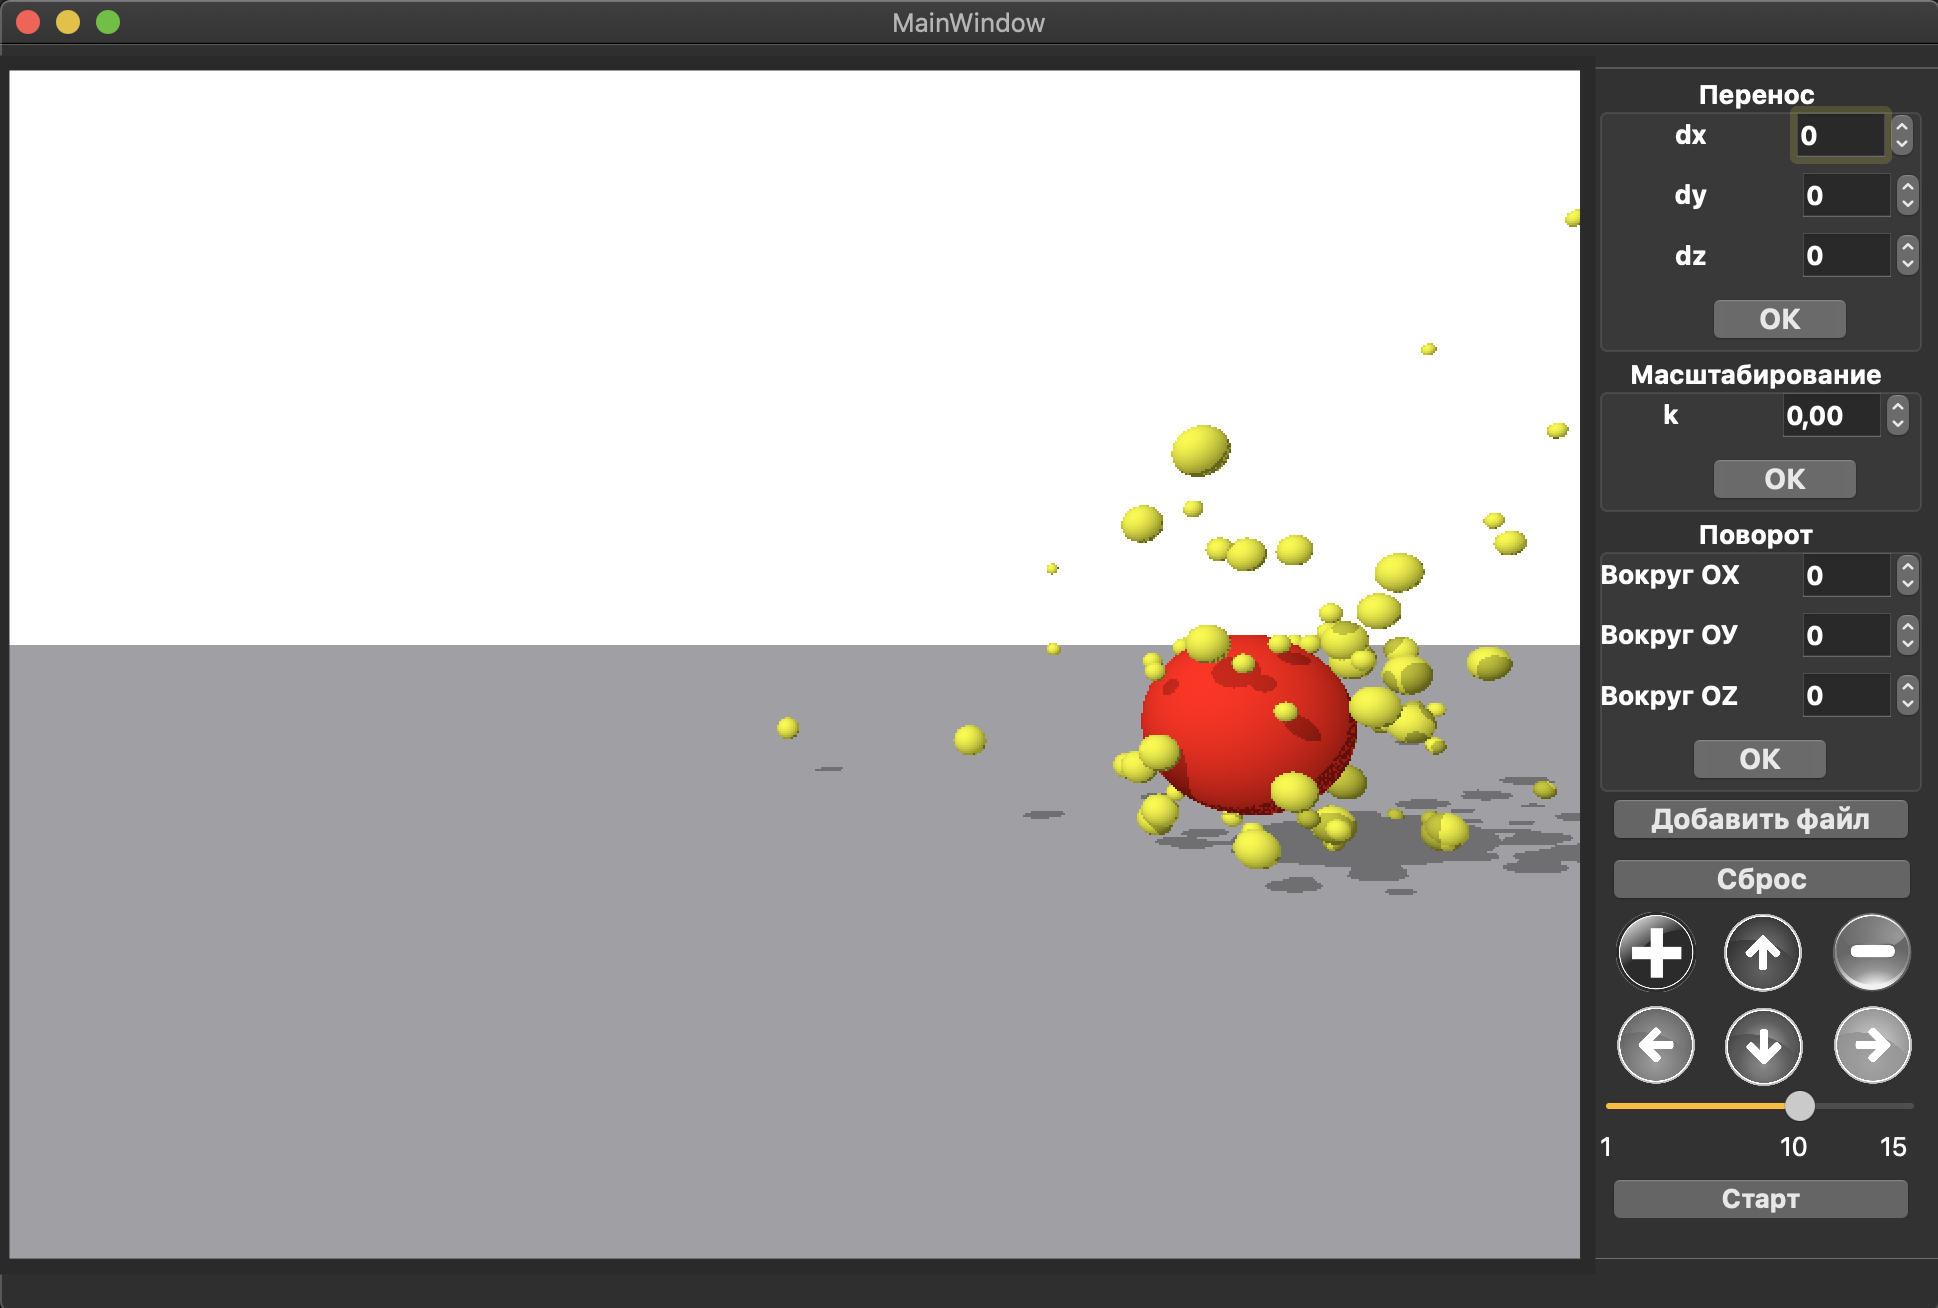
\includegraphics[scale=0.4]{ex2}
	\caption{Пример 2}
	\label{img:ex2}
\end{figure}

\section{\textbf{Вывод}}

Проведено исследование, зависимости количества частиц от времени визуализации для различного числа потоков. Получены выводы, что оптимальное число используемых потоков, при количестве частиц большем 50, равно количеству логических ядер процессора. А так как, в данной работе ставится задача визуализации взаимодействия большого числа частиц, то использовано 8 потоков. 